\documentclass[letterpaper,12pt]{report}
\usepackage[english]{babel}							%For internationalization
\usepackage[utf8]{inputenc}							%For character encoding
\usepackage{amsmath}								%For mathematical typesetting
\usepackage{amssymb}								%For mathematical typesetting
\usepackage{graphicx}								%For handling graphics
\usepackage[top=1in, bottom=1in, left=1.5in, right=1in]{geometry}	%Sets required thesis margins
\usepackage[nodisplayskipstretch,doublespacing]{setspace} 		%Sets required thesis double spacing
\usepackage{titlesec} 								%Used to easily redefine section title styles

\newcommand{\be}{\begin{equation}}
\newcommand{\ben}[1]{\begin{equation}\label{#1}}
\newcommand{\ee}{\end{equation}}
\newcommand{\aomega}{\overset{\sim}{\omega}}				%Approximate omega

\title{Vortex Dominated Flows: A High-Order, Conservative Eulerian Simulation Method}
\author{Josh Bevan}
\date{\today}

%Set section formats so chapters, sections, and subsections are 14ish pt
\titleformat{\section}{\large\bfseries}{\thesection}{1em}{}
\titleformat{\subsection}{\normalsize\bfseries}{\thesubsection}{1em}{}
\titleformat{\chapter}{\large\bfseries}{\thechapter}{1em}{}
	\titlespacing*{\chapter}{0pt}{.7in}{0pt} %Add whitespace above chapter title to get a 2in margin

%Frontmatter----------------------------------------------------------------------
\begin{document}
\pagenumbering{roman} %Roman numbering for frontmatter
\maketitle
\begin{abstract}
\setcounter{page}{2} %Manual page numbering because 'abstract' is annoying
\thispagestyle{plain} %Needed to show page number as pagestyle was reset to 'empty' when \maketitle is called internally
A high-order, conservative Eulerian method will be presented for the simulation of vortex dominated inviscid fluid flows. The primitive variable incompressible Euler equations are recast in the velocity-vorticity form to explicitly enforce conservation of vorticity. The advection of the vorticity is then calculated via a two-step process: the velocity field is first determined by evaluation of the Biot-Savart integral, and then a line-based discontinuous Galerkin (DG) Eulerian spatial discretization scheme is applied to accurately advect the vorticity field. The accuracy and convergence of this method is examined for test cases where an analytical solution exists, as well as more challenging test cases which lack an analytical solution. The influence the velocity field discretization has on the performance of the method is of particular interest.
\end{abstract}

\setcounter{page}{3} %Manual page numbering because 'abstract' is annoying
\chapter*{Acknowledgments}
\begin{singlespace} %Tables should be single spaced
\tableofcontents
\listoftables
\addcontentsline{toc}{section}{List of Tables}
\listoffigures
\addcontentsline{toc}{section}{List of Figures}
\end{singlespace}

%Here we change the pagestyle so that the page number appears top right. We need to redefine the \chapter command to change the default pagestyle from 'plain' to 'myheadings'
\pagestyle{myheadings}
\makeatletter
\renewcommand\chapter{\if@openright\cleardoublepage\else\clearpage\fi
                    \thispagestyle{myheadings}% original style: plain
                    \global\@topnum\z@
                    \@afterindentfalse
                    \secdef\@chapter\@schapter}
\makeatother

%Mainmatter-----------------------------------------------------------------------
\chapter{Introduction}
\pagenumbering{arabic} %Reset to arabic numbering for mainmatter
\section{Velocity-Vorticity equation}
Direct solution of Navier-Stokes is impractical for many fluid problems and where possible simplifications should be made; one such possibility is for vortex dominated flows. It is possible to recast Navier-Stokes from a primitive variable form ($u,v,p$) to a velocity-vorticity ($u,v,\omega$) form. This has several advantages: explicit conservation of vorticity, elimination of pressure, and reduction of required simulated DOFs to just those that form the vorticity support. For inviscid and incompressible flows the vorticity transport equation is:
\ben{VV3D} \frac{\partial \omega}{\partial t} + u \cdot \nabla \omega - \omega \cdot \nabla u = S(x,t)\ee

Traditionally simulation techniques take advantage of Helmholtz and Kelvin's theorems; vorticity exists as material surfaces, lines, etc. and therefore a Lagrangian approach is natural. Typically the vorticity is discretized into vortex particles, lines, or sheets at which point advection becomes trivial, one merely needs to calculate the velocity field at each particle and step forward in time \cite{Strain1996,MoussaCarley2008,KoumLeonard1995}. Several monographs exist that enumerate the details and advantages of Lagrangian vortex methods \cite{Lugt1983,Saffman1992,Speziale1987}.

\section{Lagrangian Methods}
There are several variations of Lagrangian methods depending on how the vorticity is discretized; point vortex methods were the earliest with the work of Rosenhead \cite{Point1} in 2D with singular point vortices, which was later built upon and improved \cite{Point2,Point3,Point4,Point5,Point6}. Higher dimensional discretizations take the form of vortex line \cite{Line1,Line2,Line3,Line4}, sheets \cite{Sheet1,Sheet2,Sheet3}, and volumes \cite{Volumes1,Volumes2,Volumes3}.

The velocity field due to the vorticity is usually calculated from solving the Poisson problem, or through inversion of the Poisson problem via evaluation of the Biot-Savart integral. There are several challenges with evaluation of the velocity: boundary conditions in the Poisson solution method, and singularities in the Biot-Savart volume integral method. Typically Lagrangian point vortex codes de-singularize the kernel \cite{Rosenhead1930,Moore1972}. Direct summation for the velocity field has a $\mathcal{O}(N^2)$ complexity. Tree-codes \cite{LindsayKrasny2001} and Fast Multipole Methods (FMM) \cite{Strain1997} are common ways of achieving a more efficient.

The convergence of vortex methods was proven early on in 2D \cite{Convg2D} and was later extended to 3D \cite{Convg3D}.

\section{Lagrangian Method Difficulties}
Lagrangian point methods present several problems. Point disorganization can occur as the fluid evolves, this typically requires temporary meshing to recondition the discretization. This has been handled with various methods; recalculation of the quadrature weights at each time step \cite{Remesh2,Remesh3}, regridding/rezoning \cite{Remesh4}, and remeshing \cite{Remesh5} among them. Additionally, most Lagrangian approaches are limited to low order; careful point locations must be chosen and maintained through frequent remeshing etc. in order to achieve high-order convergence \cite{Strain1997}.

\section{Existing Eulerian codes}
In comparison, far less literature exists for Eulerian approaches. Chief among them is the work of Brown et al. \cite{Brown2000} who adapted the velocity-vorticity approach to a low order Finite Volume (FV) solver. Later they were able to extend their method to be accelerated via a FMM \cite{Brown2004}. However, like most FV approaches, to extend to high order solution approximations requires extended stencils that ultimately limit the geometrical freedom of the mesh. Steinhoff et al. also used an Eulerian approach, but solved a modified form of the inviscid Euler equations with "vorticity confinement" rather than the velocity-vorticity equation \cite{SteinhoffUnderhill1994}.
%
\section{Proposed Method}
\subsection{Alternate Advective Methods}
The desire to resolve fine vortical structures motivates the need for a high order solver. Considering the challenges associated with achieving a high order Lagrangian method and the preliminary success of Brown et al.'s low order method, it is natural to attempt a high order Eulerian vorticity-velocity method, but what of the spatial discretization choice?

Finite difference methods suffer from similar problems as FV with extended stencils, as well as not being explicitly conservative. A finite element approach is ill-suited to the hyperbolic nature of vorticity advection. Spectral methods are promising, but for sparse vorticity domains are less-efficient due to the global support of the harmonic bases. However, discontinuous Galerkin (DG) methods are a natural choice; they are conservative, able to take advantage of vorticity sparseness, are well-suited to handle advection via intelligent choice of a numerical flux function, and have bases with local/compact support.

For domains free of impinging bodies a hexahedral mesh with a tensor product grid of interpolation points is convenient to implement. This permits the use of a line-DG \cite{Perlman1985} approach that considerably simplifies multi-dimensional cases by allowing reuse of 1D methods. A 2D domain will be considered to evaluate whether the method is practical, as well as to limit solution times to those that are reasonable on a workstation. This has the advantage of removing the vortex stretching term and reducing the vorticity to a scalar. The resultant partial differential equation (PDE) takes on the familiar form of a scalar conservation law.

\subsection{Velocity Field Fidelity}
Unlike Lagrangian methods where advection is trivial, or Brown's method which is at low order, the necessary fidelity of the velocity field to maintain a particular global convergence rate that one would expect from the order of the vorticity field is not immediately obvious. The method by which one recovers the velocity field is decoupled from the advective solver, which has no a priori knowledge or assumptions about the quality of the velocity field approximation. 

To maintain maximum flexibility for investigative purposes and to remove as much approximation error as possible the velocity field for validation of the underlying method is calculated via direct evaluation of the BS integral.

\section{Thesis Structure}
In Chapter 2, a brief overview of the underlying theory of the velocity-vorticity formulation, velocity evaluation, the Biot-Savart  kernel and the discontinuous Galerkin method are covered. The extension of one-dimensional DG methods to 2D via a line-DG style method will also be reviewed. 

In Chapter 3 the methodology taken to construct a high-order Eulerian velocity-vorticity is covered. Formation of the semi-discrete system, along with the development of some specialized tools is addressed. A high-order velocity evaluation method is laid out, as well as some computation-saving modifications. Explicit time-stepping via a Runge-Kutta method optimized for the spectra of the DG operator is briefly reviewed. Finally a test plan is laid out for validation and investigation of the overall solver and method. 

In Chapter 4 results of the validation tests, convergence studies, and performance of the possible improvements and modifications is presented. Additionally runtime performance of the solver is examined, dependent on solver parameters, tolerances, order, etc.

In Chapter 5 the successful performance of the method and solver is presented and discussed. Additionally an un-implemented extension to the velocity evaluation via a modified Fast Multipole Method is presented. Chapter 7 points in the direction of possible expansion of the method to include additional physical behaviors and configurations, as well as several next steps that should be taken to improve the solver for practical solution of larger problems beyond what is currently possible.

Finally, Chapter 8 presents the specific implementation details necessary to implement the solver practically and efficiently. Several Matlab functions and routines are presented that either makeup the solver itself, or necessary auxiliary tools that are tangentially needed.
%------------------------------------
\chapter{Theory}
\section{Navier-Stokes: Velocity-vorticity form}
If the quantity \textit{vorticity} is defined as
\be \omega = \nabla \times u \ee
Then the traditional form of the Navier-Stokes equations can be recast, assuming an inviscid incompressible flow
\ben{VV3D} \frac{\partial \omega}{\partial t} + u \cdot \nabla \omega - \omega \cdot \nabla u = S(x,t)\ee

There are several benefits to the recast form; first, it explicitly conserves vorticity. The vorticity is recoverable from the primitive variable Navier-Stokes, but the diffusive nature of most upwinded advection means coherent vortical structures are quickly smeared. Also, frequently the distribution of the vorticity is quite sparse. The primitive variable form requires the velocity and pressure be evaluated over the whole domain.

In comparison, the velocity-vorticity form only requires velocity to be evaluated in areas of non-zero vorticity. In areas where there is no vorticity, nothing needs to be advected. The sparser and more concentrated the vorticity, the larger the gap in performance between the two forms; this is especially true in 3D domains where the scaling from surfaces to volumes gives even greater opportunity for empty local regions in the domain. 

Additionally, the primitive-variable form requires the pressure be  solved via a separate elliptic equation. The velocity-vorticity form is absent the pressure and automatically ensures satisfaction of continuity.

Restricting  to examining 2-D distributions of vorticity, several simplifications can be made. The originally vectorial vorticity becomes a scalar quantity, all vorticity is directed normal to the plane. As a result, the vortex stretching term in \eqref{VV3D} becomes zero. The only non-zero component of $\omega$ is in the z-direction, however the gradient of the velocity field is zero in the z-direction, so the product is therefore zero. The result is
\ben{VV2D} \frac{\partial \omega}{\partial t} + u \cdot \nabla \omega = S(x,t)\ee
or if instead the second term is expressed in terms of the flux of the vorticity (where $f_i(\omega)=u_i\,\omega$):
\ben{VV2D} \frac{\partial \omega}{\partial t} + \frac{\partial f}{\partial x_i}= S(x,t)\ee

\section{Velocity Field Evaluation: The Biot-Savart Integral}
We shall decide that $\omega$ is the quantity of interest in the solution method. However, if this is the case then the question must be posed: how does one determine the velocity field? For an incompressible flow
\be \nabla^2 u = -\nabla \times \omega \ee
If inverted, the Biot-Savart integral is obtained
\ben{BS} u(x^*) = \int_\Omega K(x^*,x) \times \omega(x) dx \ee
with the singular Biot-Savart kernel
\ben{BSkern} K(x^*,x) = \frac{-1}{4 \pi} \frac{x^*-x}{|x^*-x|^3} \ee

There are several important points to note that are a consequence of this inversion. First, rather than solving the Poisson equation for the entirety of the domain we choose to evaluate the velocity at some subset. For the purposes of advecting the velocity we will only need velocities near the vorticity itself. However, if the number of required velocity evaluation points is roughly proportional to the $N$ DOFs of our vorticity approximation, then it might be expected for the velocity calculations to scale as $\mathcal{O}(N^2)$.

There are numerous methods to reduce the computational complexity of similar N-body type problems to $\mathcal{O}(NlogN)$ or $\mathcal{O}(N)$. Cyclic reduction \cite{SchumannSweet1976}, tree-codes \cite{LindsayKrasny2001,BarnesHut1986}, and FMM \cite{GreengardRokhlin1987} are all possibilities. However, because the velocity field calculation method is essentially decoupled from the discretization of the PDE, there is no a priori assurance that the velocity calculated is of sufficient fidelity to ensure convergence of the overall method (let alone convergence at the order one might expect based on solely the discretization). For maximum flexibility in investigating this dependency of overall convergence on the calculated velocity field we shall eschew more efficient techniques so that we can directly control the fidelity of the velocity field.

The second point to consider regarding the Biot-Savart integral is the singular nature of the exact kernel. Lagrangian point vortex methods have the benefit that the singularity and it's associated non-physical velocities occur in a relatively small region; they assume that the advective effect of the point vortex on itself is negligble. Generally, self-influence merely results in solid body rotation. Additionally they will frequently de-singularize the kernel by introducing a core function. The classical one used is the Rosenhead-Moore kernel \cite{Rosenhead1930,Moore1972}:
\ben{RMkern} K(x^*,x) = \frac{-1}{4 \pi} \frac{x^*-x}{(|x^*-x|^2+\sigma^2)^{3/2}} \ee

The high-order Eulerian approach taken here however means that the Biot-Savart integral diverges everywhere within any of the extended vorticity patches thanks to self-influence. The approach taken by Brown \cite{Brown2004} was to use the Rosenhead-Moore kernel, choosing a core size such that the maximum velocity occurred on the face of the finite volume unit. This is constructible a priori because the vorticity is taken as constant across the volume, as is typical in a FV approach. If the vorticity is spatially varying however, the choice of core size is more troublesome. This will be examined in greater detail in the next chapter.

\section{Discontinuous Galerkin}
In order to solve \eqref{VV2D} we adopt a method-of-lines approach. We will first spatially discretize the system to obtain the semi-discrete system, then we use an explicit time discretization method to march forward in time. Note that \eqref{VV2D} has the form of a scalar conservation law, with $\omega$ being the conserved quantity. The velocity field that advects the conserved quantity has been calculated by evaluation of the Biot-Savart integral for the current timestep.

Our spatial discretization is at best an approximate solution to \eqref{VV2D}, that we shall denote as $\aomega(x,t)$. Some residual will remain for the approximate solution of the PDE at any time $t$
\ben{VV2D} \frac{\partial \aomega}{\partial t} + \frac{\partial f}{\partial x_i} = R(x)\ee
where we have shown a 1-D case and omitted vorticity sources for simplicity.

The discontinuous Galerkin (DG) approach attempts to approximately satisfy the PDE in the following way: Seek the best approximation in a finite vector test space $\mathbb{W}_h$  in the $L^2$ norm sense. Minimize the $L^2$ norm by an orthogonal projection of the residual onto $\mathbb{W}_h$. Form a complete basis for $\mathbb{W}_h$ with a set of test functions $\phi_j \in \mathbb{W}_h$, such that the orthogonal projection satisfies:
\be \int_\Omega R(x) \phi_j \;dx = 0 \quad\mbox{for all}\; j\ee
Substituting the residual for our conservation PDE yields:
\be \int_\Omega \frac{\partial \aomega}{\partial t} \, \phi_j \;dx + \int_\Omega \frac{\partial f(\aomega)}{\partial x} \, \phi_j \;dx = 0 \quad\mbox{for all}\; j\ee

Choose the space of piecewise polynomials for the finite dimensional approximation space, and decompose the global domain into K elements where the local approximation space $\overset{k}{\mathbb{V}}_h$ has basis functions $\overset{k}{\psi}_i(x)$ over the local domain $x \in [x_L, x_R]$ (henceforth we drop the element index $k$ for brevity, except when describing two distinct elements that must be distinguished). Note that continuity of vorticity is not enforced across elements, and that the local approximation spaces for each element are independently defined. Finally, take the Bubnov-Galerkin choice of setting the test space to be the same as the approximation space so that $\phi_j=\psi_i \in \mathbb{V}_h$ if $i=j$. The local Mth order approximation to vorticity takes the form

\be \omega(x,t) \approx \aomega(x,t) = \sum_{i=0}^M a_i(t)\psi_i(x)\ee

where $a_i$ is some set of coefficients that are to be determined. The elemental approximating PDE is then

\be \sum_{i=0}^M \left[ \frac{d a_i(t)}{dt}\int_{x_L}^{x_R}\psi_i(x)  \, \phi_j(x) \;dx \right]
+ \int_{x_L}^{x_R} \frac{\partial f(\aomega)}{\partial x} \, \phi_j \;dx = 0 \ee

To reduce the smoothness requirements on the flux, integrate the second term by parts to yield
\ben{DGtemp} \sum_{i=0}^M \left[ \frac{d a_i(t)}{dt}\int_{x_L}^{x_R}\psi_i(x)  \, \phi_j(x) \;dx \right]
+ f\phi_j(x) \Big|^{x_R}_{x_L} 
- \int_{x_L}^{x_R} f(\aomega) \, \frac{d \phi_j(x)}{d x} \;dx = 0 \ee

The local solution offers no way of recovering the global solution, until one realizes that the flux at the element boundaries is multiply defined between elements. The global solution is allowed to be piecewise discontinuous across boundaries, so there is no guarantee that the flux between neighboring elements would agree. To resolve this (and at the same time recover a global solution) define a numerical flux analogous to a Finite Volume Method that takes as input the vorticity at the adjacent element boundaries. We will use an upwind flux, where defining the average as $\{\!\{\omega^+\}\!\} = \frac{\omega^++\omega^-}{2}$ and the jump as $[[\omega]]=\omega^+-\omega^-$, yields
\be \hat{f}_{upwind}(x^+,x^-)=u\{\!\{\aomega\}\!\} + \frac{|u|}{2}[[\aomega]]\ee

We would also like to map any element to a computational element by means of a mapping $x=g(X)$ and it's inverse $X=G(x)$. If we set the domain of our computational element to be $X \in [-1, 1]$ and the element size to be $\Delta x = x_R - x_L$, then the mapping is
\be x=g(X)=\frac{X+1}{2}\Delta x + x_L\quad ,\quad X=G(x)=\frac{2(x-x_L)}{\Delta x}+1 \ee

Applying a change of variables using the mapping to \eqref{DGtemp}, accounting for the numerical flux, and being sure to include the determinant of the Jacobian matrix that results from the mapping ($J=g'(X)=\Delta x/2$) in the first integral:
\ben{DGtemp} \frac{\Delta x}{2}	\sum_{i=0}^M \left[ \frac{d a_i}{dt}	\int_{-1}^{1}\psi_i  \, \phi_j \;dX \right]
+\hat{f}\phi_j \Big|^{x_R}_{x_L} 
- \int_{-1}^{1} f(\aomega) \, \frac{d \phi_j}{dX} \;dX = 0 \ee
(Note: no determinant of the Jacobian matrix appears in the second integral because one of the basis functions has been differentiated. When the chain rule is applied during the change of variables an extra $1/g'(X)$ appears that cancels out with the $g'(X)$ that occurred from the change of variables on the integral).

We have purposely left the flux in the second integral unevaluated in terms of the basis functions, as well as the choice of basis functions left as undecided. We defer these choices to a more in depth investigation in Methodology. We also have developed the equations past the initial PDE in a 1-D form. We will shortly show that the basis coefficients are chosen to be nodal values. The 2-D solution will be recovered following the Line-DG methodology \cite{Persson2013} element will be composed of a tensor product of two 1-D discretization.

%------------------------------------
\chapter{Methodology}
\section{Overall Solver Structure}
IC and BC initialization, Lagrange pre-calculation, mass and stiffness matrices generation, 2 step spatial discretization, time discretization, post processing
\newpage.
\newpage
\section{Use and Abuse of Structured Tensor Mesh}
\newpage
\section{Mass Matrix}
\section{Modified Quadrature}
\newpage
\section{Stiffness Matrix Integration}
\newpage.
\newpage
\section{Velocity Evaluation}
\newpage
\section{Vortex Sparseness}
\section{Reduced Order Velocity (Global)}
\newpage
\section{Reduced Order Velocity (Far-field)}
\newpage
\section{Explicit Time-Stepping}
\newpage
\section{Validation and Convergence of Proposed Methods}
(analytical cases, elliptical blob, 2-D "ring",several interacting patches) vs (convergence rate of: constant order velocity field, linear far field velocity [far= 1 element or X element separation], variable far field velocity order [heuristic?])

The method will be validated via comparison with test cases for which analytical solutions exist (Perlman \cite{Perl} test case, stationary isentropic vortex, elliptical patch \cite{Koum}), as well a replication of empirical results from test cases \cite{Emp}. The qualitative performance of the method will also be evaluated with more complex test cases, including the collision of two vortex pairs, "leap-frogging", and several arbitrary patch configurations.
\newpage

%------------------------------------
\chapter{Results}
\section{Analytical Test Cases}
\newpage.
\newpage.
\newpage.
\newpage
\section{Elliptical Blob}
\newpage.
\newpage.
\newpage
\section{Arbitrary Patch}
\newpage.
\newpage.
\newpage
\section{Vortex Pair}
\newpage.
\newpage.
\newpage
\section{Vortical System}
\newpage.
\newpage.
\newpage
\section{Reduced Order Velocity}
\newpage.
\newpage.
\newpage
\section{Runtime Speed and Memory Footprint of Solver}
%------------------------------------
\chapter{Discussion}
\section{Analytical Validation of Model}
Comparison of existing analytical solutions vs model (Euler vortex, 5th order poly, other Saffmann test cases)
\newpage.
\newpage
\section{Empirical Convergence of Method}
\newpage.
\newpage
\section{Computational Efficiency}
\newpage.
\newpage
\section{Extended Body Fast Multipole Formulation}
%------------------------------------
\chapter{Conclusion}
%------------------------------------
\chapter{Recommendations}
\section{Extension to 3D}
\section{Flux Limiters}
\section{Impinging Geometry and Boundary Conditions}
\section{Viscosity}
\newpage
\section{Implicit and Local Time Stepping}
\section{Parallelizability}
\section{FMM Improvements}
\section{2D Non-classical Quadrature for Nearly Singular Integrands}
%------------------------------------
\chapter{Implementation and Algorithms}
\section{Modified Two-part quadrature}
Vectorized Lagrange evaluation, Lagrange derivatives, etc
\newpage
\section{Binary Singleton Expansion Matrix-Vector Products}
\section{Lagrange Bases and Constructed Quadrature}
\newpage
\section{Velocity Evaluation}
\section{Semi-discrete System Construction}
\newpage
\section{Low-storage Stability Optimized Runge-Kutta}
%------------------------------------
\chapter{Literature Cited}
\begin{thebibliography}{9}
%Overview
\bibitem{Lugt1983}
H. J. Lugt, Vortex Flow in Nature and Technology, Krieger Publishing Company, Malabar, FL, USA, 1983.
\bibitem{Saffman1992}
P. G. Saffman, Vortex Dynamics, Cambridge Univ. Press, Cambridge, UK, 1992.
\bibitem{Speziale1987}
C. G. Speziale, On the advantages of the vorticity-velocity formulation of the equations of fluid dynamics, J. Comput. Phys. 73 (1987) 476-480.
%Point methods
\bibitem{Point1}
L. Rosenhead, The formation of vorticies from a surface of discontinuity, Proc. Roy. Soc. London Ser. A 134 (1931) 170-192.
\bibitem{Point2}
G. Birkhoff, J. Fisher, Do vortex sheets roll up?, Rend. Circ. Math. Palermo, Ser. 2 8 (1959) 77-90.
\bibitem{Point3}
F. H. Abernathy, R. E. Kronauer, The formation of vortex streets, J.Fluid Mech. 13 (1962) 1-20.
\bibitem{Point4}
A. J. Chorin, P. S. Bernard, Discretization of a vortex sheet, with an example of roll-up, J. Comput. Phys. 13 (3) (1973) 423-429.
\bibitem{Point5}
K. Kuwahara, H. Takami, Numerical studies of two-dimensional vortex motion by a system of point vortices, J. Physical Society of Japan 34 (1) (1973) 247-253.
\bibitem{Point6}
R. G. Zalosh, Discretized simulation of vortex sheet evolution with buoyancy and surface tension effects, AIAA Journal 14 (11) (1976) 1517-1523.
%Line methods
\bibitem{Line1}
G. K. Batchelor, An Introduction to Fluid Dynamics, Cambridge University Press, 1967, 1973.
\bibitem{Line2}
W. T. Ashurst, E. Meiburg, Three-dimensional shear layers via vortex dynamics, J. Fluid Mech. 189 (1988) 87-116.
\bibitem{Line3}
J. E. Martin, E. Meiburg, Numerical investigation of three-dimensional evolving jets subject to axisymmetric and azimuthal perturbation, J. Fluid Mech. 230 (1991) 271-318.
\bibitem{Line4}
A. Leonard, Numerical simulation of interacting, three-dimensional vortex filaments, in: Proceedings of the IV Intl. Conference on Numerical Methods of Fluid Dynamics, no. 35 in Lecture Notes in Physics, Springer-Verlag, 1975, pp. 245-250.
%Sheet methods
\bibitem{Sheet1}
M. E. Agishtein, A. A. Migdal, Dynamics of vortex surfaces in three dimensions: Theory and simulations, Physica D 40 (1989) 91-118.
\bibitem{Sheet2}
O. M. Knio, A. F. Ghoniem, Three-dimensional vortex simulation of rollup and entrainment in a shear layer, J. Comput. Phys. 97 (1991) 172-223.
\bibitem{Sheet3}
O. M. Knio, A. F. Ghoniem, Vortex simulation of a three-dimensional reacting shear layer with in finite-rate kinetics, AIAA J. 30 (1) (1992) 105-116.
%Volume methods
\bibitem{Volumes1}
G. Russo, J. A. Strain, Fast triangulated vortex methods for the 2D Euler equations, J. Comput. Phys. 111 (1994) 291-323.
\bibitem{Volumes2}
M. Carley, A triangulated vortex method for the axisymmetric Euler equations, J. Comput. Phys. 180 (2002) 616-641.
\bibitem{Volumes3}
S. A. Huyer, J. R. Grant, Solution of two-dimensional vorticity equation on a Lagrangian mesh, AIAA Journal 38 (5) (2000) 774-783.
%Remeshing problems
\bibitem{Strain1996}
J. Strain. 2D vortex methods and singular quadrature rules. Journal of Computational Physics 124.1 (1996): 131-145.
\bibitem{Remesh2}
J. T. Beale, On the accuracy of vortex methods at large times, in: IMA Workshop on Computational Fluid Dynamics and Reacting Gas Flows, Springer-Verlag, 1988, p. 19.
\bibitem{Remesh3}
J. S. Marshall, J. R. Grant, Penetration of a blade into a vortex core: vorticity response and unsteady blade forces, J. Fluid Mech. 306 (1996) 83-109.
\bibitem{Remesh4}
H. O. Nordmark, Rezoning for higher order vortex methods, J. Comput. Phys. 97 (1991) 366-397.
\bibitem{Remesh5}
H. N. Najm, R. B. Milne, K. D. Devine, S. N. Kempa, A coupled Lagrangian-Eulerian scheme for reacting flow modeling, ESAIM Proc. 7 (1999) 304-313.
%Convergence
\bibitem{Convg2D}
O. H. Hald, V. D. Prete, Convergence of vortex methods for Euler's equations, Math. Comput. 32 (1978) 791-809.
\bibitem{Convg3D}
J. T. Beale, A convergent 3-D vortex method with grid-free stretching, Math. Comput. 46 (174) (1986) 401-424.

%Brown
\bibitem{Brown2000}
 R.E. Brown. Rotor Wake Modeling for Flight Dynamic Simulation of Helicopters. AIAA Journal, 2000. Vol. 38(No. 1): p. 57-63.
\bibitem{Brown2004}
A.J. Line, R.E. Brown. Efficient High-Resolution Wake Modelling using the Vorticity Transport Equation. in 60th Annual Forum of the American Helicopter Society. 2004. Baltimore, MD.\bibitem{Persson2013}
P.O. Persson. A Sparse and High-Order Accurate Line-Based Discontinuous Galerkin Method for Unstructured Meshes. J. Comp. Phys., Vol. 233, pp. 414-429, Jan 2013.
\bibitem{Strain1997}
J. Strain. Fast adaptive 2D vortex methods. Journal of computational physics 132.1 (1997): 108-122.
\bibitem{LindsayKrasny2001}
K. Lindsay, and R. Krasny. A particle method and adaptive treecode for vortex sheet motion in three-dimensional flow. Journal of Computational Physics 172.2 (2001): 879-907.
\bibitem{Rosenhead1930}
L. Rosenhead. The spread of vorticity in the wake behind a cylinder, Proc. Roy. Soc. London Ser. A 127, 590 (1930).
\bibitem{Moore1972}
D. W. Moore. Finite amplitude waves on aircraft trailing vortices, Aero. Quart. 23, 307 (1972).
\bibitem{Perlman1985}
M. Perlman. On the accuracy of vortex methods, J. Comput. Phys. 59 (1985) 200–223.
\bibitem{Koum1997}
P. Koumoutsakos. Inviscid axisymmetrization of an elliptical vortex, J. Comput. Phys. 138 (1997) 821–857.
\bibitem{KoumLeonard1995}
Koumoutsakos, P., Leonard, A. (1995). High-resolution simulations of the flow around an impulsively started cylinder using vortex methods. Journal of Fluid Mechanics, 296, 1-38.
\bibitem{Southerland1991}
K. B. Southerland, J. R. P. III, W. J. A. Dahm, K. A. Buch. An experimental study of the molecular mixing process in an axisymmetric laminar vortex ring, Phys. Fluids A 3 (5) (1991) 1385–1392.
\bibitem{MoussaCarley2008}
Moussa, C., Carley, M. J. (2008). A Lagrangian vortex method for unbounded flows. International journal for numerical methods in fluids, 58(2), 161-181.
\bibitem{SteinhoffUnderhill1994}
J. Steinhoff, D. Underhill, Modification of the Euler equations for "vorticity confinement": Application to the computation of interacting vortex rings, Phys. Fluids 6 (8) (1994) 2738-2743.
\bibitem{SchumannSweet1976}
Schumann, U., Sweet, R. A. (1976). A direct method for the solution of Poisson's equation with Neumann boundary conditions on a staggered grid of arbitrary size. Journal of Computational Physics, 20(2), 171-182.
\bibitem{BarnesHut1986}
Barnes, J.,  Hut, P. (1986). A hierarchical O (N log N) force-calculation algorithm.
\bibitem{GreengardRokhlin1987}
Greengard, L.,  Rokhlin, V. (1987). A fast algorithm for particle simulations. Journal of computational physics, 73(2), 325-348.
%\bibitem{}
%\bibitem{}
%\bibitem{}
%\bibitem{}
%\bibitem{}
%\bibitem{}
%\bibitem{}
%\bibitem{}
%\bibitem{}
%\bibitem{}
%\bibitem{}

\end{thebibliography}
%\begin{figure}
%\centering
%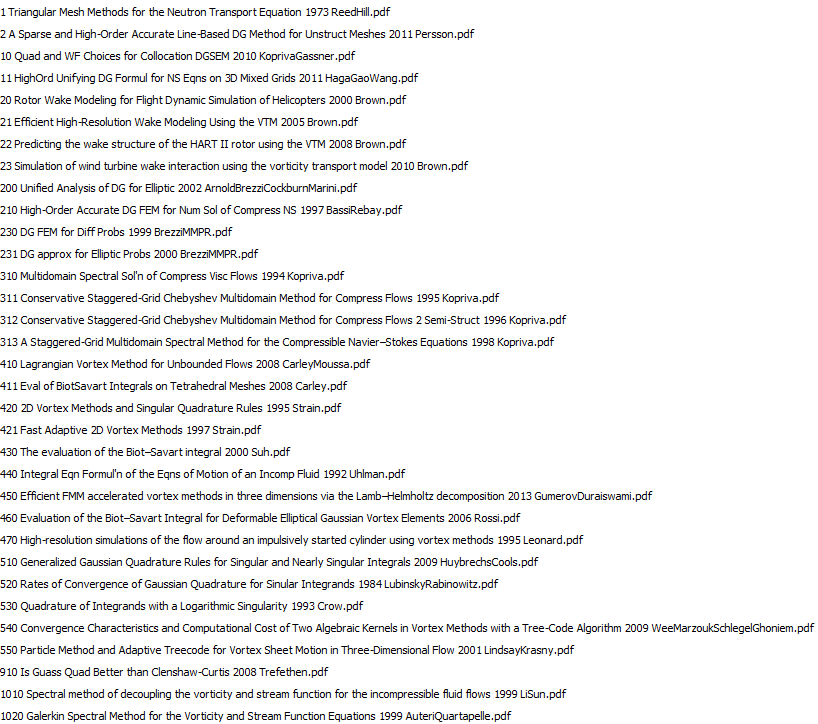
\includegraphics[width=1.4\textwidth]{LitStart.PNG}
%\caption{\label{fig:ring}Dirty preliminary lit cited.}
%\end{figure}

\end{document}